\chapter{Modelo Matemático}

Aquí va el resumen del capítulo

\newpage
\section{Descripción del sistema bajo estudio. Ecuaciones de Gobierno}

Se considera el sistema representado en la Figura \ref{fig:sistem_domain} donde la dinámica de un fluido viscoso e incompresible sucede entre dos paredes paralelas e infinitas ubicadas en $y=-d$ y $y=+d$. Esto constituye un canal de placas paralelas donde ambas paredes están sometidas a un flujo de calor constante $q''_w$.

\begin{figure}[H]
 \centering
  \subfloat[]{
    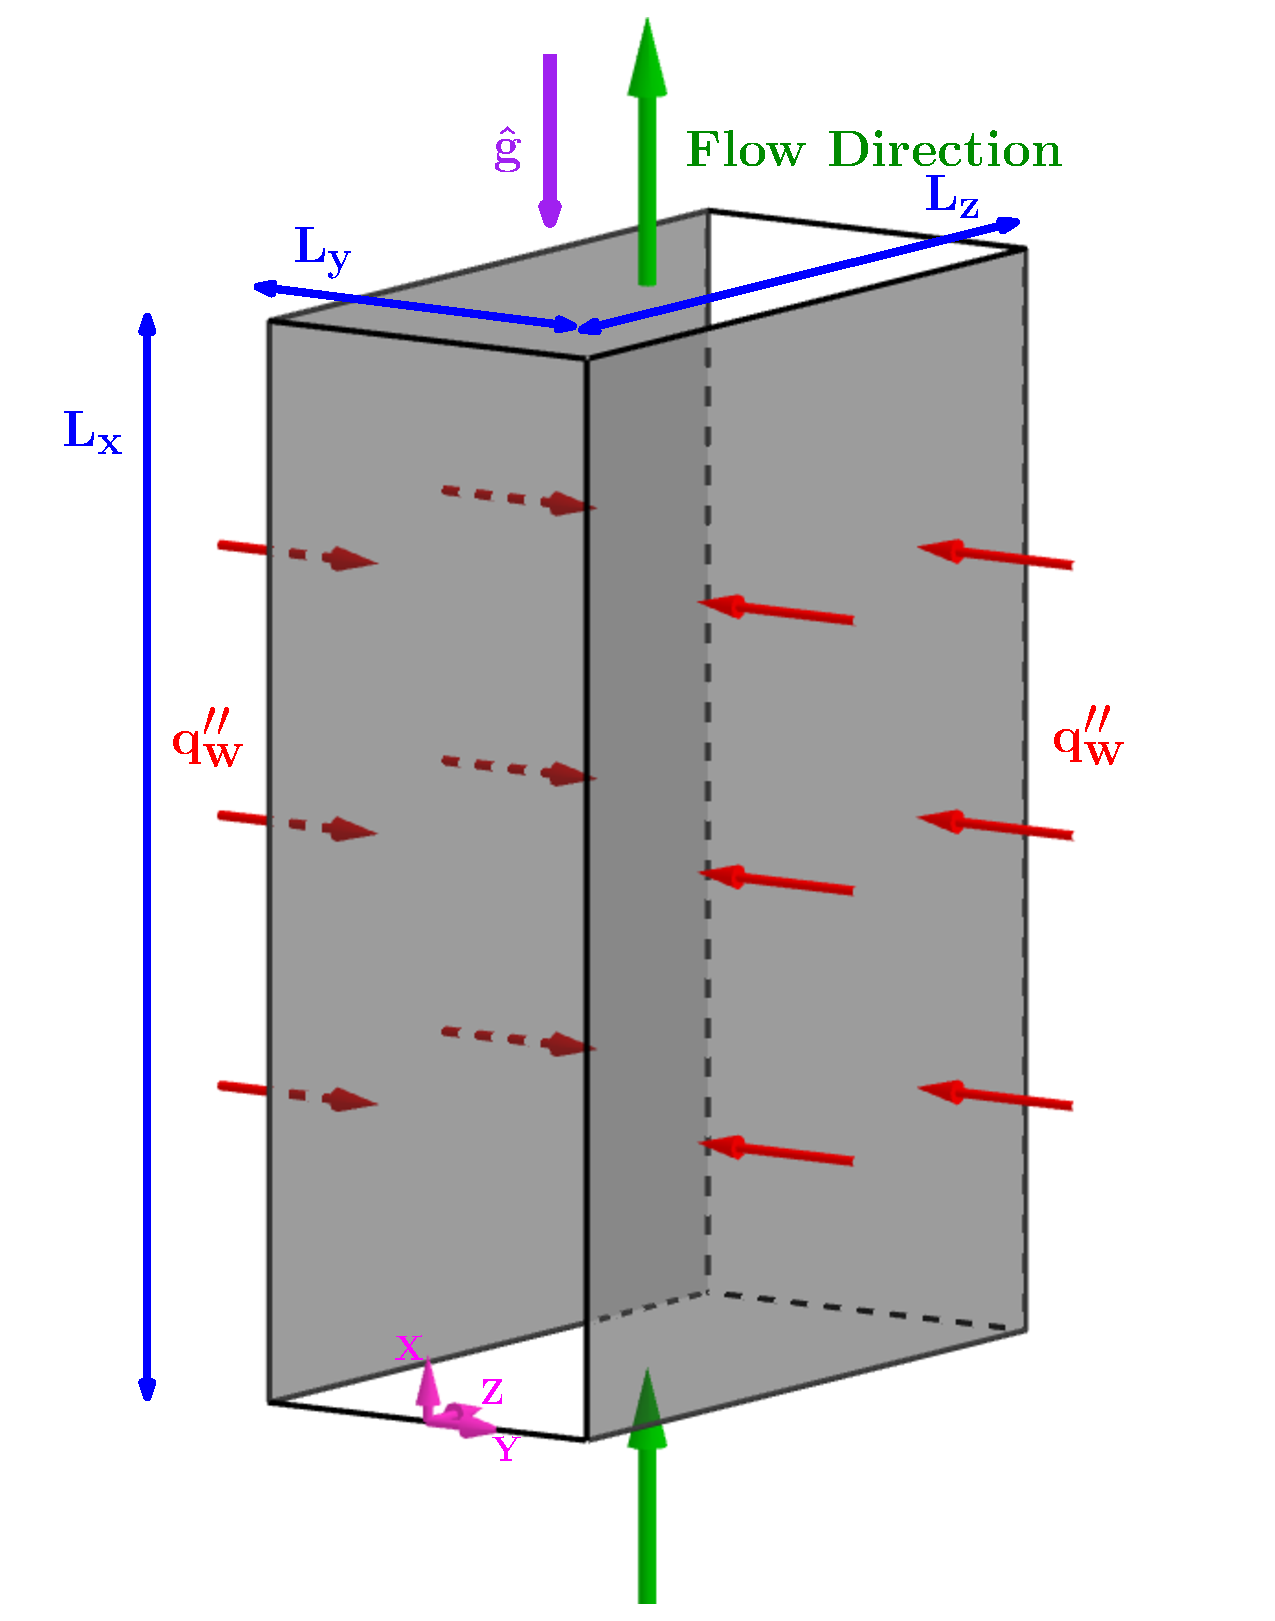
\includegraphics[width=0.49\textwidth]{figures/domain3d.eps}
    \label{fig:dom3d}}  
    \subfloat[]{
    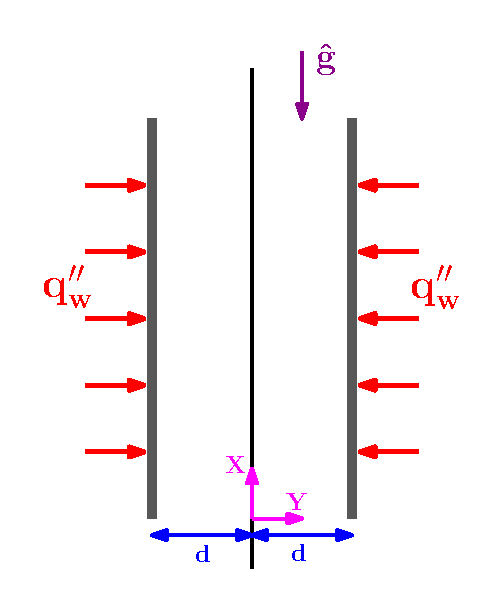
\includegraphics[width=0.49\textwidth]{figures/domain2d.eps}
    \label{fig:dom2d}}  
 \caption{} 
 \label{fig:sistem_domain}
\end{figure}


La dirección del flujo se encuentra en la dirección de la corriente (\textit{stramwise}) paralelo al eje X y su sentido es opuesto a la aceleración de la gravedad. Las ecuaciones de gobierno corresponden a los principios de conservación de masa, momento y energía que se expresan en el cuadro \ref{eq:gob_system}.

\begin{equation}
        \boxed{ \begin{array}{lcc}
			  %\\
              &  \nabla \cdot \left( \rho_o \mathbf{u} \right) = 0 \\
              \vspace*{2mm}
              &  \frac{\partial \left( \rho_o \mathbf{u} \right)}{\partial t} + \mathbf{u} \cdot \nabla  \left( \rho_o \mathbf{u} \right) = -\nabla \text{p} + \mu \hspace{1mm} {\nabla}^2 \mathbf{u}  + \rho(T) \hspace{1mm} \mathbf{g} \\
              \vspace*{2mm}
              &  \frac{\partial T}{\partial t} + \mathbf{u} \cdot \nabla T =  \alpha \hspace{1mm} \nabla^2 T  \\
              % \\
             \end{array}
               }
             \label{eq:gob_system}
\end{equation}

Un sistema físico cuyas dimensiones ``son muy grandes'' (o infinitas) constituye un sistema ideal. En él, es posible ubicar el origen de nuestro sistema de referencia lejos de los extremos a fin de evitar efectos de bordes. Allí, el flujo se encuentra completamente desarrollado y ha alcanzado un estado estadísticamente estacionario, es decir, sus valores estadísticos, como el promedio, no varían en el tiempo. En este contexto, la condición de flujo de calor constante en las paredes se imponen como condiciones de Neumann:

\begin{equation}
\kappa \hspace{0.5mm} \left. \frac{\partial T}{\partial y} \right\vert_{y=\mp d} = \pm q''_w
\label{eq:neumann}
\end{equation}

Sin embargo, debido a la limitación computacional evidente, nuestro modelo computcional no puede abarcar dicha extensión. En ese sentido, el ``dominio infinito'' se reemplaza con un dominio acotado de dimensiones $L_x \times L_y \times L_z$ (Figura \ref{fig:dom3d}) adoptando condiciones de borde periódicas (PBC) en la direcciones $X$ y $Z$:
\begin{align}
\eta(x=0,y,z,t) &= \eta(x=L_x,y,z,t) \\ 
\eta(x,y,z=0,t) &= \eta(x,y,z=L_z,t)
\end{align}
siendo $\eta$ un campo escalar de interés. Esto se puede interpretar como si las PBC crearan ``la ilusión'' de un dominio infinito, mediante la repetición de este dominio finito en el espacio.

Por otra parte, en un flujo turbulento, dado que este no es estacionario, aparecen fluctuaciones del flujo de calor y de la temperatura sobre la superficie de la pared. En este contexto, Kasagi et al. \cite{kasagi1992direct} asumen que las fluctuaciones de temperatura son pequqeñas a fin de considerar que la temperatura en la pared es localmente isotérmica y que además, el flujo de calor no varía en la dirección de la corriente. Esto es equivalente a suponer que la temperatura en la pared, promediada en el tiempo y en la dirección $Z$, crece linealmente con $x$, y por lo tanto: 

$$
\langle T_w \rangle = A \hspace{0.5mm} x.
$$

Debido al crecimiento lineal de $\langle T_w \rangle$, es requerido realizar el cambio de variable $T(x,y,z,t) = \langle T_w \rangle - \theta(x,y,z,t)$ para que siga siendo válido las condiciones de borde periódicas, esto es, $\theta(x=0,y,z,t)=\theta(x=L_x,y,z,t)$. Dicha modificación introduce un término fuente en la ecuación de conservación de energía:

\begin{equation}
\frac{ \partial \theta }{ \partial t } + \mathbf{u} \cdot \nabla \theta = \alpha \nabla^2 \theta + A \hspace{0.5mm} u_x 
\label{eq:energy_pcb_source}
\end{equation}
Por su parte, el término $\rho(T) \mathbf{g}$ en la ecuación de momento se reescribe empleando la aproximación de Bousinessq \cite{incropera}, $\rho(T) = \rho_o \left[ 1 - \beta (T - T_R) \right]$:

\begin{equation}
\frac{ \rho_o \hspace{0.5mm} \partial \mathbf{u}}{\partial t} + \mathbf{u} \cdot \nabla  \left( \rho_o \mathbf{u} \right) = -\nabla \left( \text{p} + \rho_o \hspace{0.5mm} g \hspace{0.5mm} x \right) + \mu \hspace{1mm} {\nabla}^2 \mathbf{u}  + g \hspace{1mm} \rho_o \hspace{1mm} \beta \hspace{1mm} \theta \hspace{1mm} \mathbf{\hat{g}}   
\end{equation}
donde se ha considerado $T_R = \langle T_w \rangle$, siendo $\mathbf{\hat{g}}=(-1,0,0)$.

Mediante el balance de energía en el volumen de control $L_x \times L_y \times L_z$, es posible deducir que $A = \frac{q''_w}{\rho_o  d \langle u \rangle c_p}$ siendo $d$ el semiancho del canal. Así, empleando la velocidad en el centro del canal $U_o$, el semiancho $d$ y la temperatura $T_c = A \hspace{0.3mm} d $, el sistema de ecuaciones \ref{eq:gob_system} en su forma adimensional queda escrito como se muestra en el cuadro \ref{eq:gob_system_adim}. 

Otro detalle importante es el hecho de que el fluido de trabajo es impulsado por un caudal másico constante. Esta cuestión se encuentra representada por el término fuente $f \mathbf{\hat{x}}$, en la ecuación de momento, donde $f$ es una constante en el espacio y varía con el tiempo de manera que mantiene constante el caudal total. 

\begin{equation}
\boxed{
\begin{array}{l}
    \nabla^* \cdot \mathbf{u^*} = 0 \\
    \frac{\partial \mathbf{u^*}}{\partial t^*} + \mathbf{u^*} \cdot \nabla^* \mathbf{u^*} = 
    -\nabla \text{p}^* + \frac{1}{\text{Re}_o} \hspace{0.5mm} \nabla^{*2} \mathbf{u^*} + \text{Ri}_o \hspace{0.5mm} \theta^* \hspace{0.5mm} \mathbf{\hat{g}} + f \mathbf{\hat{x}} \\
    \frac{\partial \theta^*}{\partial t^*} + \mathbf{u^*} \cdot \nabla^* \theta^* = 
    \frac{1}{\text{Pr}}\hspace{0.5mm}  \frac{1}{\text{Re}_o} \hspace{0.5mm} \nabla^{*2} \theta^* + u_x^* 
\end{array}
}
\label{eq:gob_system_adim}
\end{equation}

$$\text{Re}_o = \frac{\mu}{\rho_o \hspace{0.5mm} U_o\hspace{0.5mm} d } \quad ; \quad \text{Pr}= \frac{\nu_o}{\alpha} \quad ; \quad \text{Ri}_o = \frac{g \beta \Delta T d}{U_o^2} = \frac{\text{Ra}}{\text{Re}_o^2 \hspace{1mm} \text{Pr}}$$
%siendo Ra, el número de Rayleigh.

Asimismo, las condiciones de flujo de calor constante están expresadas en la ecuación \ref{eq:neumann_adim}. Sin embargo, estas condiciones pueden ser aproximadas como condiciones de Dirichlet ya que al suponer que la temperatura de las paredes es constante, fluctuaciones igual a cero, se obtiene: $T(x,y=0,z,t) = T(x,y=2d,z,t) = \langle T_w \rangle$. Su forma adimensional se expresa en la ecuación \ref{eq:dirichlet_adim_theta}. Por otra parte, para el resto de variables (campo de presión y componentes de velocidad) se adoptan condiciones de no deslizamiento en las paredes. 

\begin{align}
\begin{array}{l}
    \left. \frac{\partial \theta^*}{\partial y^*} \right\vert_{y^*=-1} = + \frac{2}{3} \text{Re}_o \hspace{0.5mm} \text{Pr} \\
    \left. \frac{\partial \theta^*}{\partial y^*} \right\vert_{y^*=+1} = - \frac{2}{3} \text{Re}_o \hspace{0.5mm} \text{Pr} 
\end{array}
\label{eq:neumann_adim}
\end{align}

\begin{equation}
\theta^*(x^*,y^*=0,z^*,t^*) = \theta^*(x^*,y^*=2,z^*,t^*) = 0
\label{eq:dirichlet_adim_theta}
\end{equation}





\section{Teoría de Estabilidad Lineal. Perturbaciones} \label{line_an}

Para analizar la estabilidad lineal y prever de forma matemática cómo cambiará un flujo una vez perturbado, resulta indispensable aceptar que las perturbaciones actúan sobre un flujo base. Aquí se adopta como referencia el flujo laminar completamente desarrollado. En consecuencia, la evolución de las perturbaciones también queda condicionada por dicho estado inicial.



\section{Flujo Base}

Si el flujo está completamente desarrollado, térmica e hidrodinámicamente, entonces el mismo solo dependerá de la variable $y^*$. El sistema de ecuaciones \ref{eq:gob_system_adim} se reduce a la ecuación de momento en la dirección $X$ y a la ecuación de transporte del escalar pasivo, las cuales quedan expresadas como 

\begin{equation}
\frac{d \text{p}^* }{d x^*} = \frac{\text{Ra}}{\text{Re}^2 \hspace{1mm} \text{Pr}} \theta^* + \frac{1}{\text{Re}} \frac{d^2 u^*_x}{d {y^*}^2}
\label{eq:base1}
\end{equation}

\begin{equation}
\frac{d^2 \theta^*}{ d {y^*}^2 } = - {\text{Pr}} \hspace{1mm} \text{Re} u^*_x
\end{equation}
El perfil de velocidad y de temperatura admiten las condiciones de borde $u^*_x({y^*}= \pm 1) = \theta^* ({y^*}= \pm 1) = 0 $. Las soluciones para un flujo asistido por fuerzas boyantes están dadas por las expresiones \ref{eq:vel_asist_boyant} y \ref{eq:theta_asist_boyant}, mientras que para un flujo donde las fuerzas boyantes son opuestas, las soluciones quedan definidas por las ecuaciones \ref{eq:vel_opo_boyant} y \ref{eq:theta_opo_boyant} \cite{chen1996linear}. 
\small{
\begin{equation}
U_x = \frac{-E}{\sqrt{\text{Ra}}} \frac{\sinh(\kappa(1+y^*))\sin(\kappa(1-y^*)) + \sinh(\kappa(1-y^*))\sin(\kappa(1+y^*)) }{\cosh(2\kappa) + \cos(2\kappa)}
\label{eq:vel_asist_boyant}
\end{equation}

\begin{equation}
\Theta^* = \frac{E}{\text{Ra}} \left[ 1 - \frac{\cosh(\kappa(1+y^*))\cos(\kappa(1-y^*)) + \cosh(\kappa(1-y^*))\cos(\kappa(1+y^*))}{\cosh(2\kappa) + \cos(2\kappa)} \right] 
\label{eq:theta_asist_boyant}
\end{equation}


\begin{equation}
U_x = \frac{F}{2 m^2} \left( \frac{\cosh(m y^*)}{\cosh(m)} - \frac{\cos(m y^*)}{\cos(m)} \right) 
\label{eq:vel_opo_boyant}
\end{equation}

\begin{equation}
\Theta^* = \frac{F}{2 m^4} \left( \frac{\cosh(m y^*)}{\cos(m)} + \frac{\cos(m y^*)}{\cos(m)} - 2 \right) 
\label{eq:theta_opo_boyant}
\end{equation}

\begin{equation*}
\kappa = \frac{\text{Ra}^{-1/4}}{\sqrt{2}} \quad ; \quad m = (-\text{Ra})^{1/4} \quad ; \quad F = \frac{2 m^3}{\tanh(m)-\tan(m)} \quad ; \quad
\end{equation*}

\begin{equation*}
E= -2 \kappa \hspace{1mm} \text{Ra}^{1/2} \hspace{1mm} \frac{\cosh(2\kappa) + \cos(2\kappa)}{\sinh(2\kappa) - \sin(2\kappa)} 
\end{equation*}
}
donde $\Theta^*= \frac{-1}{\text{Re} \hspace{1mm} \text{Pr}} \theta^*$ y $U_x = \frac{2}{3} u^*_x$. Obsérvese que el único parámetro aquí es el número de Rayleigh.
 
En el Capitulo 3, se utilizarán estás ecuaciones para la validación de la herramienta numérica en estas condciones. 

\section{Análsis de Estabilidad Lineal}

La transición laminar-turbulenta, es decir, la evolución de un flujo laminar a uno turbulento, es crucial en ingeniería, ya que las características del flujo varían notablemente entre estos regímenes. Por ejemplo, los coeficientes de fricción y de convección aumentan considerablemente al pasar de un régimen laminar a uno turbulento. La ecuación de Navier–Stokes admite ambas soluciones bajo ciertos parámetros, lo que implica que el tipo de flujo y su evolución dependen de las perturbaciones y las condiciones impuestas en el sistema. Muchos fenómenos que cumplen exactamente las leyes de conservación resultan inobservables porque se inestabilizan ante las pequeñas perturbaciones inevitables en cualquier sistema real \cite{kundu}.

El análisis de estabilidad lineal permite evaluar cómo se comporta un flujo ante perturbaciones, identificando los mecanismos que pueden inducir transiciones o estados de intermitencia. En el caso de flujos de fluidos, condiciones como un número de Reynolds inferior a un valor crítico garantizan la estabilidad de un flujo laminar suave. Sin embargo, en ocasiones las perturbaciones crecen hasta alcanzar amplitudes finitas y establecer nuevos equilibrios estacionarios, que pueden volverse inestables a su vez y evolucionar hacia estados de fluctuaciones caóticas, comúnmente descritos como turbulencia. Dos motivaciones principales para estudiar la estabilidad de los fluidos son comprender el proceso de transición de un flujo laminar a uno turbulento y predecir el inicio de dicha transición.

El enfoque parte de las ecuaciones de gobierno \ref{eq:gob_system_adim}. La idea consiste en suponer que los campos solución ($\mathbf{u^*}$,$\text{p}^*$,$\theta^*$) pueden descomponerse como un flujo base más una perturbación:


\begin{align}
\mathbf{u^*} &= \mathbf{U} + \tilde{\mathbf{u}}^* \\
\text{p}^* &= \text{P}+ \tilde{\text{p}}^* \\
\theta^* &= \Theta + \tilde{\theta}^*
\end{align}  
donde las letras mayusculas hacen referencia al flujo base y aquellas letras con $\tilde{()}$ a las perturbaciones. Asimismo, se asume que $\mathbf{u^*}$, $\text{p}^*$, $\mathbf{U} = (U_x,U_y,U_z)$ y $\text{P}$ satisface el sistema \ref{eq:gob_system_adim}. Así, despreciando

\\